%----------------------------------------------------------------------------------------
%    PACKAGES AND THEMES
%----------------------------------------------------------------------------------------

\documentclass[aspectratio=169,xcolor=dvipsnames]{beamer}
\usetheme{SimplePlus}

\usepackage{hyperref}
\usepackage{graphicx} % Allows including images
\usepackage{booktabs} % Allows the use of \toprule, \midrule and \bottomrule in tables
\usepackage{appendixnumberbeamer}
\usepackage[font=small]{caption}
\usepackage{algorithm}
\usepackage{algpseudocode}

\usepackage{natbib}
\usepackage{amssymb}
\usepackage{amsmath}
\usepackage{amsthm}
\usepackage{nicefrac}       % compact symbols for 1/2, etc.
\usepackage{microtype}      % microtypography
\usepackage{caption}
\usepackage{subcaption}
\usepackage{xfrac}
\usepackage{soul}
\usepackage{wasysym}
\usepackage{tabularx}
\usepackage{multicol}

% ====================
% Lengths
% ====================

% If you have N columns, choose \sepwidth and \colwidth such that
% (N+1)*\sepwidth + N*\colwidth = \paperwidth

\newcommand{\defeq}{\stackrel{\text{def}}{=}}
\newcommand{\bh}{\mathbf{h}}
\newcommand{\bt}{\mathbf{t}}
\newcommand{\bu}{\mathbf{u}}
\newcommand{\bv}{\mathbf{v}}
\newcommand{\bw}{\mathbf{w}}
\newcommand{\bx}{\mathbf{x}}
\newcommand{\bz}{\mathbf{z}}
\newcommand{\by}{\mathbf{y}}

\newcommand{\bA}{\mathbf{A}}
\newcommand{\bC}{\mathbf{C}}
\newcommand{\bI}{\mathbf{I}}
\newcommand{\bT}{\mathbf{T}}
\newcommand{\bW}{\mathbf{W}}
\newcommand{\bX}{\mathbf{X}}
\newcommand{\bZ}{\mathbf{Z}}

\newcommand{\bepsilon}{\boldsymbol{\epsilon}}
\newcommand{\bmu}{\boldsymbol{\mu}}
\newcommand{\blambda}{\boldsymbol{\lambda}}
\newcommand{\bsigma}{\boldsymbol{\sigma}}
\newcommand{\bSigma}{\boldsymbol{\Sigma}}

\newcommand{\bbE}{\mathbb{E}}
\newcommand{\bbP}{\mathbb{P}}
\newcommand{\bbQ}{\mathbb{Q}}
\newcommand{\bbR}{\mathbb{R}}
\newcommand{\bbW}{\mathbb{W}}

\newcommand{\mbbP}{\mathbb{P}_{\text{MCMC}}}

\newcommand{\cL}{\mathcal{L}}
\newcommand{\cN}{\mathcal{N}}
\newcommand{\cS}{\mathcal{S}}
\newcommand{\cT}{\mathcal{T}}
\newcommand{\cX}{\mathcal{X}}
\newcommand{\cB}{\mathcal{B}}
\newcommand{\cA}{\mathcal{A}}
\newcommand{\cY}{\mathcal{Y}}
\newcommand{\cP}{\mathcal{P}}
\newcommand{\cF}{\mathcal{F}}
\newcommand{\cW}{\mathcal{W}}
\newcommand{\cE}{\mathcal{E}}
\newcommand{\cU}{\mathcal{U}}
\newcommand{\cV}{\mathcal{V}}
\newcommand{\cM}{\mathcal{M}}
\newcommand{\cZ}{\mathcal{Z}}
\newcommand{\cH}{\mathcal{H}}

\newcommand{\cmark}{\ding{51}}
\newcommand{\xmark}{\ding{55}}

\newcommand{\red}[1]{\textcolor{red}{#1}}
\newcommand{\green}[1]{\textcolor{Green}{#1}}

\newcommand{\E}[2][]{\bbE_{#1}\!\left[ #2 \right]}
\newcommand{\EX}[3][]{\tilde \bbE^{#2}_{#1}\!\left[ #3 \right]}
\newcommand{\EXD}[2][]{\EX[#1]{\alpha}{#2}}

%----------------------------------------------------------------------------------------
%    TITLE PAGE
%----------------------------------------------------------------------------------------

\title{Revisiting the L\'evy Foraging Hypothesis in 2D with Reproducible Simulation}
\subtitle{Thesis Pre-defence}

\author{Anita Toleutaeva \inst{1} }

\institute{%
    \inst{1} Skolkovo Institute of Science and Technology
}

\date{}

%----------------------------------------------------------------------------------------
%    PRESENTATION SLIDES
%----------------------------------------------------------------------------------------

\begin{document}

\begin{frame}
    % Print the title page as the first slide
    \titlepage
\end{frame}

\begin{frame}{Background: Random Search}
Sparse-target blind search (limited cues).

\textbf{L\'evy flights} - heavy-tailed step-length random walk (power-law).
\begin{figure}[h]
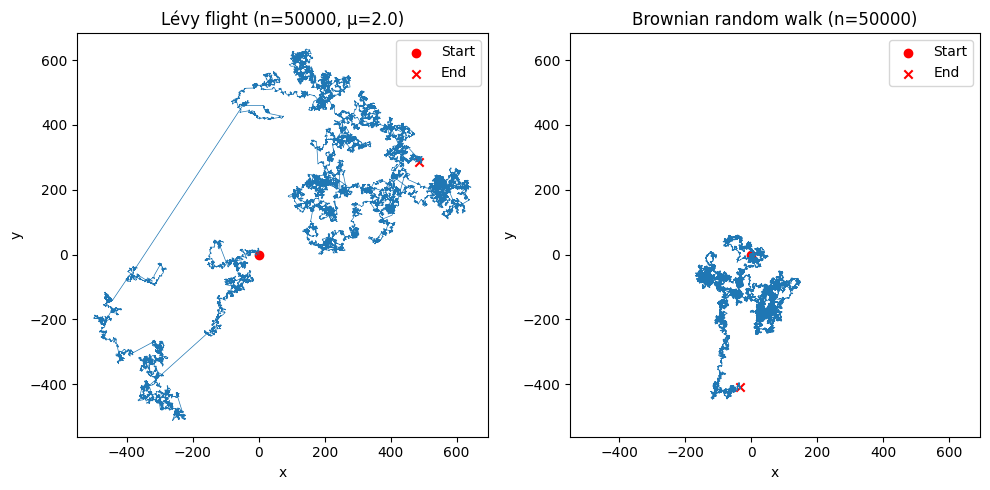
\includegraphics[width=0.7\linewidth]{figs/levy_brownian1.png}
\caption{L\'evy (Cauchy) and Brownian trajectories of different lengths.}
\end{figure}
\end{frame}


\begin{frame}{Problem: the L\'evy foraging hypothesis}
\begin{block}{}
    \centering
    \textbf{Claim (Viswanathan et al., 1999):} inverse-square L\'evy flights ($\mu \approx 2$) maximise encounter rates in sparse environments.
\end{block}
\vspace{6pt}
\begin{block}{}
    \centering
    Is $\mu^* = 2$ truly universal across densities and post-detection strategies, or is it an artifact of specific modeling assumptions?
\end{block}
\vspace{4pt}
\begin{multicols}{2}
\textbf{Why it matters}
\begin{itemize}
    \item Biology: interpreting animal movement data and foraging optimality.
    \item Robotics: efficient exploration/search without maps.
    \item Theory: resolving contradictory ``L\'evy optimality'' results.
\end{itemize}

\columnbreak
\textbf{Why timely}
\begin{itemize}
\item Mature debate + high-quality critiques exist, but a \textbf{unified benchmark is missing.}
\end{itemize}
\end{multicols}
\end{frame}


\begin{frame}{L\'evy flights and the search model}
\textbf{L\'evy flights:} random walks with power-law distributed step lengths.
\begin{itemize}
    \item $\mu \to 1$: ballistic (long straight flights)
    \item $\mu = 2$: inverse-square (``L\'evy optimal'')
    \item $\mu \to 3$: Brownian-like (diffusive)
\end{itemize}
\vspace{6pt}
\textbf{Viswanathan model:}
\begin{itemize}
    \item 2D infinite plane, homogeneous Poisson targets at density $\rho$, detection radius $r_v$.
    \item Mean free path $\lambda = 1/(2\rho r_v)$; sparsity $\lambda/r_v$.
    \item Flight length: $p(l) \propto l^{-\mu}$, \quad $l \in [l_{\min},\, l_{\max}]$.
    \item Destructive vs.\ non-destructive post-detection strategies.
\end{itemize}
\end{frame}

% why is it important?
\begin{frame}{Goals and objectives}
\begin{block}{}
    \centering
    \textbf{The aim of this work} is to construct a reproducible 2D simulation benchmark and to determine quantitatively under which conditions the inverse-square L\'evy exponent $\mu^* = 2$ is optimal, when the optimum shifts to ballistic or Brownian-like regimes, and how sensitively $\mu^*$ depends on the post-detection strategy, target sparsity, and truncation parameters.
\end{block}
\textbf{Objectives}:
\begin{itemize}
    \item \textbf{Build a reproducible 2D simulator} with truncated power-law flights ($\mu \in [1, 3]$), destructive and non-destructive search.

\item \textbf{Sweep key factors:} $\mu$, target density $\rho$ (via sparsity $\lambda/r_v \in [10, 2000]$), and four post-detection strategies.

\item \textbf{Measure efficiency metrics:} pooled unique-capture rate $\eta$ and MFPT; assess statistical convergence.

\item \textbf{Construct the phase diagram $\mu^*(\lambda/r_v)$} across all strategies.
\end{itemize}
\end{frame}

\begin{frame}{Evidence Supporting L\'evy Optimality}
    Multiple experimental and theoretical papers claim L\'evy optimality: efficiency peaks at $\mu \approx 2$ for destructive search in sparse Poisson fields \cite{viswanathan1999optimizing,raposo2003dynamical,bartumeus2002optimizing}.

\begin{figure}[h]
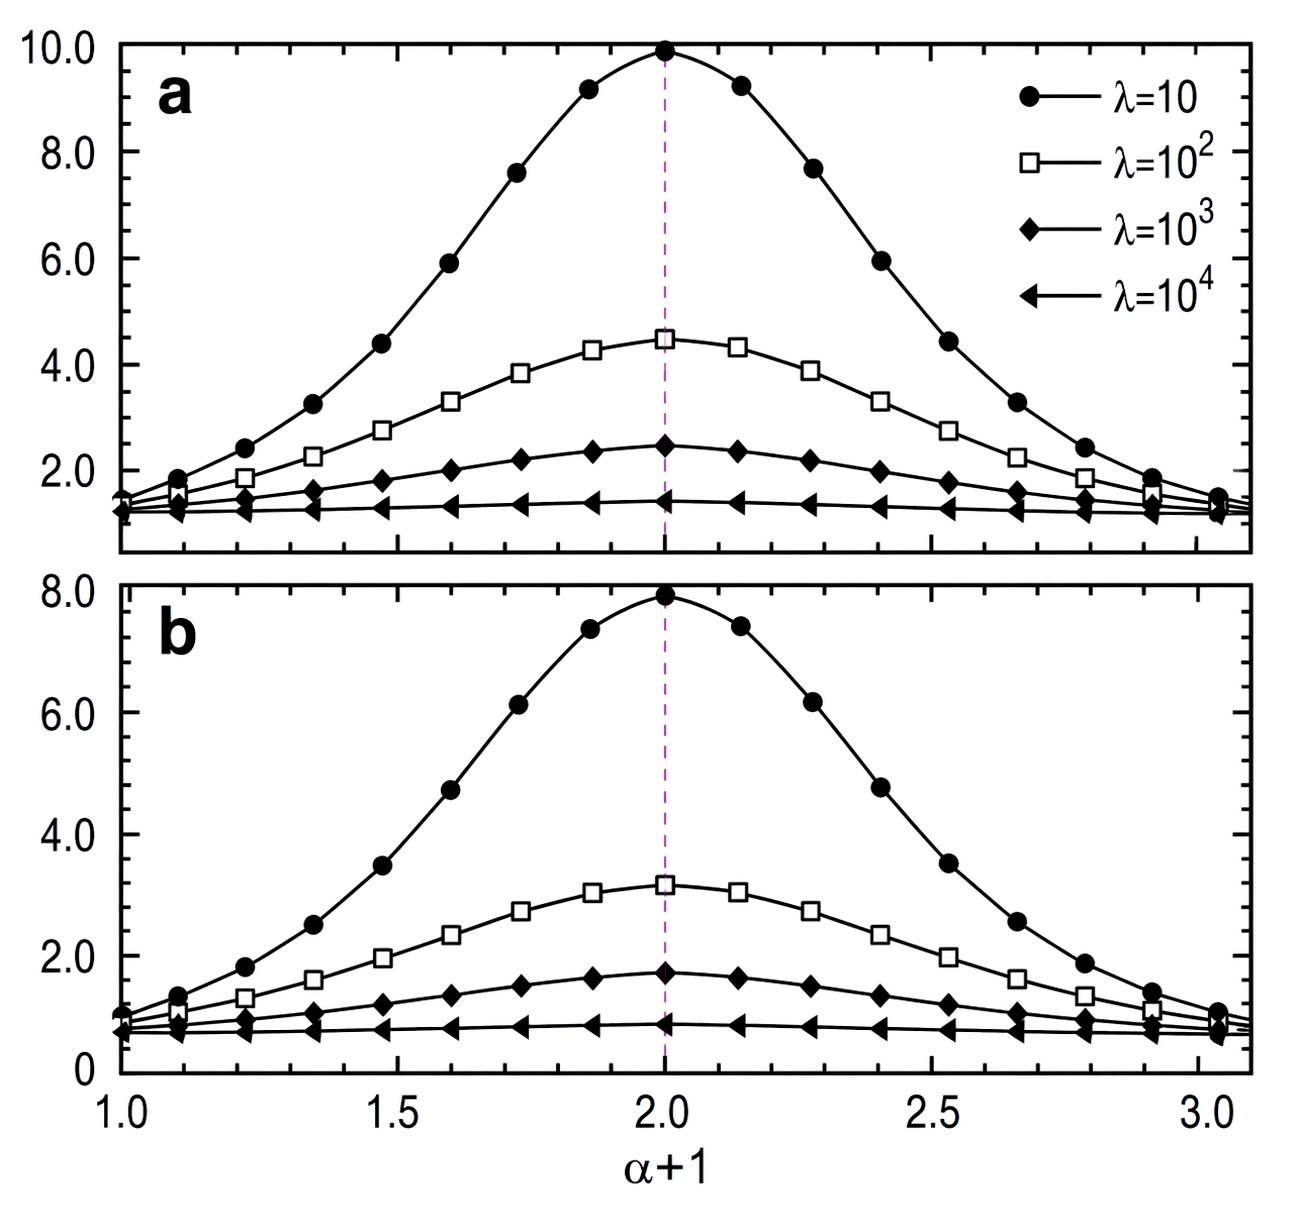
\includegraphics[width=0.35\linewidth]{figs/viswanathan1999.png}
\caption{$\lambda\eta$ vs.\ $\mu$ (from Viswanathan et~al., 1999).  Peak near $\mu = 2$.}
\end{figure}

\end{frame}

\begin{frame}{Contradictions and Context Dependence}
\textbf{Empirical re-analyses} \cite{edwards2007revisiting}:
\begin{enumerate}
    \item Likelihood-based model selection favors gamma or composite Brownian over pure power laws.
    \item Apparent power-law behavior can arise from data pooling and segmentation.
\end{enumerate}
\textbf{Theoretical critiques}:
\begin{enumerate}
    \item \cite{palyulin2014levy}: drift/flows can make Brownian/ballistic better than L\'evy for MFPT.
    \item \cite{levernier2020inverse}: in $d\geq 2$, encounter rate scales linearly with $\rho$ for all $\mu$; optimality is a prefactor effect.
    \item \cite{buldyrev2021comment}: reset distance $l_c$ and destructive vs.\ non-destructive rules qualitatively change the optimum.
\end{enumerate}

\begin{block}
    \centering
    Optimal $\mu$ is highly sensitive to drift, boundaries, and microscopic reset rules.
\end{block}
\end{frame}



\begin{frame}{Approach overview}
    \begin{enumerate}
        \item 2D infinite plane with chunked PPP target generation.
        \item Four post-detection strategies (destructive and non-destructive):
        \begin{itemize}
            \item No interrupt, Teleport ($l_c = 5r_v$), Viswanathan destructive, Viswanathan non-destructive.
        \end{itemize}
        \item Sweep $\mu \in [1,3]$ from ballistic ($\mu \to 1$) through L\'evy ($\mu \approx 2$) to Brownian ($\mu \to 3$) at each density.
    \end{enumerate}
    \begin{figure}[h]
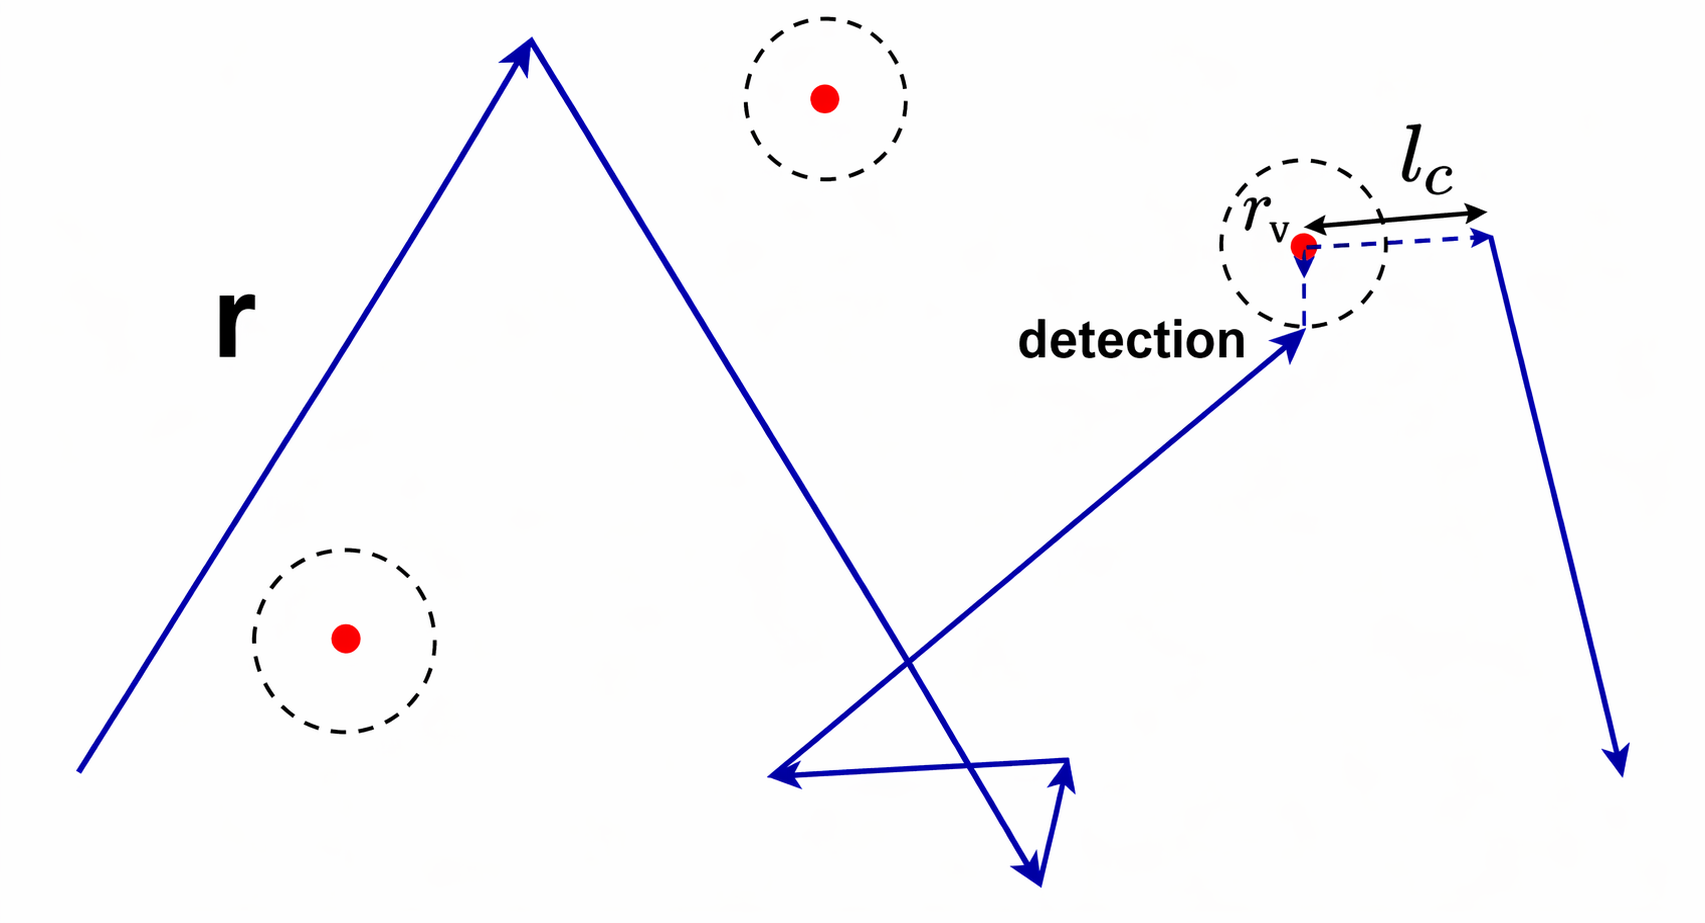
\includegraphics[width=0.4\linewidth]{figs/chart3.jpg}
\caption{The L\'evy walk search model and its parameters (Levernier, N).}
\end{figure}
\end{frame}


%========================================================================================
%    METHODOLOGY
%========================================================================================

\begin{frame}{Simulation setup}
\begin{multicols}{2}
\textbf{Model}
\begin{itemize}
    \item Targets: homogeneous PPP, density $\rho$
    \item Flights: $p(l) \propto l^{-\mu}$, $l \in [l_{\min}, l_{\max}]$
    \item Detection: corridor of width $2r_v$
    \item Mean free path: $\lambda = 1/(2\rho r_v)$
    \item Sparsity: $\lambda/r_v = 1/(2\rho r_v^2)$
\end{itemize}

\columnbreak
\textbf{Efficiency metric}
\[
\eta = \frac{\sum_{r} N_{\text{unique}}^{(r)}}{\sum_{r} D_{\text{total}}^{(r)}}
\]
Pooled (global) estimator --- robust to heavy-tailed per-run fluctuations.

\vspace{8pt}
Normalized: $\lambda\eta$ (dimensionless).
\end{multicols}

\vspace{5pt}
\footnotesize
\begin{tabular}{lcccc}
\toprule
$\lambda/r_v$ & $\rho$ & Steps/run & Runs (destr.) & Runs (non-d.) \\
\midrule
10--50   & 0.04--0.2  & 20k--30k   & 100 & 300 \\
100--500 & 0.004--0.02 & 50k--80k  & 120 & 360 \\
1000--2000 & 0.001--0.002 & 100k--150k & 120 & 360 \\
\bottomrule
\end{tabular}
\end{frame}

%========================================================================================
%    RESULTS
%========================================================================================

\begin{frame}{Phase diagram: $\mu^*(\lambda/r_v)$}
\begin{columns}[T]
\begin{column}{0.55\textwidth}
\begin{figure}

\includegraphics[width=\linewidth]{figs/phase_diagram_mu_star_clean.png}
\caption{Optimal L\'evy exponent $\mu^*$ vs.\ sparsity for all four strategies.}
\end{figure}
\end{column}
\begin{column}{0.43\textwidth}
\textbf{Key findings:}
\begin{itemize}
    \item $\lambda/r_v \geq 500$: all strategies $\to$ $\mu^* \approx 2.0$ \green{$\checkmark$}
    \item $\lambda/r_v = 10$--$20$: three strategies shift toward $\mu^* = 1.0$--$1.4$ (ballistic)
    \item Non-destructive Viswanathan: $\mu^* \approx 2.2$--$2.6$ at high $\rho$ (trapping artifact)
\end{itemize}
\vspace{8pt}
\begin{block}{}
    \centering
    $\mu^* \approx 2$ confirmed in sparse limit.

    At high density: ballistic is optimal.
\end{block}
\end{column}
\end{columns}
\end{frame}

\begin{frame}{Phase diagram: $\mu^*(\lambda/r_v)$ --- with uncertainty}
\begin{columns}[T]
\begin{column}{0.55\textwidth}
\begin{figure}

\includegraphics[width=\linewidth]{figs/phase_diagram_mu_star.png}
\caption{Same data with $\pm 1\sigma$ uncertainty bands.}
\end{figure}
\end{column}
\begin{column}{0.43\textwidth}
\textbf{Uncertainty bands:}
\begin{itemize}
    \item Shaded regions: all $\mu$ where $\eta(\mu) \geq \eta(\mu^*) - \sigma$.
    \item At $\lambda/r_v \geq 100$: narrow bands $\to$ well-determined $\mu^*$.
    \item At $\lambda/r_v = 10$: wide bands $\to$ exponent matters less.
\end{itemize}
\end{column}
\end{columns}
\end{frame}

\begin{frame}{Efficiency curves $\lambda\eta(\mu)$}
\begin{figure}
\centering

\includegraphics[width=0.85\linewidth]{figs/eta_curves_by_sparsity.png}
\caption{$\lambda\eta(\mu)$ at three sparsity levels.  Shaded bands: $\pm 1\sigma$ per-run.}
\end{figure}
\vspace{-5pt}
\begin{itemize}
    \item At $\lambda/r_v = 2000$: sharp peak at $\mu \approx 2$; all strategies $\to \lambda\eta_{\max} \approx 0.51$.
    \item At $\lambda/r_v = 10$: curves nearly flat --- $\mu$ matters little.
\end{itemize}
\end{frame}

% Slides 12--13 moved to appendix (mu* table + trapping heatmap)


\begin{frame}{Mean first passage time (MFPT)}
\begin{columns}[T]
\begin{column}{0.48\textwidth}
\begin{figure}

\includegraphics[width=\linewidth]{figs/mfpt_vs_mu.png}
\caption{MFPT$/\lambda$ vs.\ $\mu$ (destructive Viswanathan).}
\end{figure}
\end{column}
\begin{column}{0.48\textwidth}
\begin{figure}

\includegraphics[width=\linewidth]{figs/mfpt_comparison_lrv100.png}
\caption{MFPT comparison at $\lambda/r_v = 100$.}
\end{figure}
\end{column}
\end{columns}
\vspace{5pt}
\begin{itemize}
    \item MFPT minimum near $\mu \approx 1.5$ at $\lambda/r_v = 100$ --- lower than the throughput optimum ($\mu^* \approx 1.7$).
    \item Non-destructive Viswanathan: highest MFPT due to trapping.
\end{itemize}
\end{frame}


%========================================================================================
%    SUMMARY AND CONCLUSIONS
%========================================================================================

\begin{frame}{Comparison with Previous Work}
Our results at $\lambda/r_v \geq 500$ confirm the central prediction of Viswanathan et~al.\ (1999), with $\mu^* = 1.8$--$2.0$ across all four strategies. The qualitative observation by Bartumeus et~al.\ (2005) that the L\'evy advantage weakens at high density is now quantified: the crossover from L\'evy-optimal ($\mu^* \approx 2$) to ballistic-optimal ($\mu^* \to 1$) occurs at $\lambda/r_v \approx 50$--$200$, depending on the strategy.

\vspace{6pt}
The scaling critique of Levernier et~al.\ (2020), that in $d \geq 2$ the exponent affects only prefactors, is consistent with our observation that $\lambda\eta$ varies by only a factor of~${\sim}2$ across $\mu \in [1,3]$ even in the sparse limit. The non-destructive Viswanathan results (with effective $l_c = 0$) show trapping pathology rather than the clean optimum predicted by Buldyrev et~al.\ (2021), highlighting extreme sensitivity to the restart mechanism.
\end{frame}


\begin{frame}{Summary and Conclusions}
As a result of our work, we can draw the following conclusions. The optimal L\'evy exponent converges to $\mu^* \approx 2$ in the sparse-target limit ($\lambda/r_v \geq 500$) for all four strategies, confirming the L\'evy foraging hypothesis under the conditions where it was originally formulated. However, at high target density ($\lambda/r_v \leq 20$), the optimum shifts to $\mu^* \to 1$ (ballistic) for all strategies except non-destructive Viswanathan, where ``ping-pong'' trapping (${\sim}10^3$ revisits per unique target) creates a spurious shift of $\mu^*$ above~$2$.

\vspace{6pt}
The MFPT-optimal exponent ($\mu \approx 1.5$) is shifted toward ballistic values compared to the throughput optimum ($\mu^* \approx 1.7$), confirming that these two objectives select for different strategies. The standard truncation $l_{\min} = r_v$, $l_{\max} = \lambda$ is robust, with $\mu^*$ insensitive to moderate variations of these bounds.
\end{frame}


\begin{frame}{Possible Future Directions}
The present study suggests several natural extensions. A complete MFPT phase diagram across all sparsity levels and strategies would clarify whether the throughput--MFPT gap persists at extreme sparsity. Extending the simulation to three dimensions would test whether quantitative crossover densities change, since the detection geometry (cylinder vs.\ corridor) introduces new scaling. Replacing the Poisson field with clustered distributions would probe the robustness of the phase diagram against realistic spatial correlations.

\vspace{6pt}
Varying the restart distance~$l_c$ from~$0$ to $\gg r_v$ would map the full phase diagram in the $(l_c, \lambda/r_v)$ plane. Incorporating energy-aware metrics could shift the optimum at high density, and comparing with reinforcement-learning agents~\cite{munozgil2023optimal} would quantify how close the power-law family is to the true optimum.
\end{frame}


% -------------------- References slide --------------------
\begin{frame}{References}
    % Core baseline and empirical critique
    \nocite{viswanathan1999optimizing}
    \nocite{edwards2007revisiting}

    % Positive / supporting results
    \nocite{bartumeus2002optimizing}
    \nocite{raposo2003dynamical}
    \nocite{benichou2011intermittent}

    % Critical / contradictory theory
    \nocite{palyulin2014levy}
    \nocite{levernier2020inverse}
    \nocite{buldyrev2021comment}

    % Evolutionary / empirical support
    \nocite{wosniack2017evolutionary}
    \nocite{humphries2012foraging}

    % Learning / active-matter approaches
    \nocite{munozgil2023optimal}
    \nocite{kaur2023adaptive}

    \tiny
    \bibliography{reference.bib}
    \bibliographystyle{apalike}
\end{frame}


\begin{frame}
    \LARGE{\centerline{\textbf{Thank you!}}}
\end{frame}

%========================================================================================
%    APPENDIX
%========================================================================================
\appendix

\begin{frame}{Appendix: Convergence analysis}
\begin{columns}[T]
\begin{column}{0.48\textwidth}
\begin{figure}

\includegraphics[width=\linewidth]{figs/convergence_flights.png}
\caption{Convergence in number of flights (120 reps).}
\end{figure}
\end{column}
\begin{column}{0.48\textwidth}
\begin{figure}

\includegraphics[width=\linewidth]{figs/convergence_reps.png}
\caption{Convergence in number of runs (50k flights).}
\end{figure}
\end{column}
\end{columns}
\vspace{5pt}
\begin{itemize}
    \item Destructive: $\mu^*$ stable from $N_{\text{flights}} \geq 5000$, $R \geq 50$.
    \item Non-destructive: requires $R \geq 200$ due to trapping outliers.
    \item Production runs are well-converged ($<1.5\%$ change).
\end{itemize}
\end{frame}

\begin{frame}{Appendix: Analytical validation --- $\eta = 1/(\langle l \rangle \cdot N)$}
\begin{columns}[T]
\begin{column}{0.48\textwidth}
\begin{figure}

\includegraphics[width=\linewidth]{figs/analytical_comparison.png}
\caption{Simulation vs.\ Viswanathan (1999) at $\lambda/r_v = 100$.}
\end{figure}
\end{column}
\begin{column}{0.48\textwidth}
\begin{figure}

\includegraphics[width=\linewidth]{figs/analytical_multi_sparsity.png}
\caption{Analytical vs.\ simulation at four sparsity levels.}
\end{figure}
\end{column}
\end{columns}
\vspace{5pt}
Viswanathan (1999), eqs.\ 2--3, 5:\quad
$\eta = \dfrac{1}{\langle l \rangle_{\text{MF}} \cdot N}$,\quad
$N = \left(\dfrac{\lambda}{r_v}\right)^{(\mu-1)/2}$

\vspace{3pt}
Full formula correctly predicts the peaked shape and peak location near $\mu \approx 2$.
\end{frame}

\begin{frame}{Appendix: $\mu^*$ values across all densities}
\begin{table}
\centering
\small
\begin{tabular}{rcccc}
\toprule
$\lambda/r_v$ & No interrupt & Teleport & Visw.\ destr. & Visw.\ non-d. \\
\midrule
   10 & 1.1 & 1.0 & 1.0 & 2.2 \\
   20 & 1.4 & 1.4 & 1.2 & 2.6 \\
   50 & 1.8 & 1.8 & 1.7 & 2.6 \\
  100 & 1.9 & 1.9 & 1.7 & 2.5 \\
  200 & 1.9 & 1.8 & 1.9 & 2.0 \\
  500 & 2.0 & 1.9 & 1.8 & 1.9 \\
 1000 & 2.0 & 2.0 & 1.9 & 2.0 \\
 2000 & 2.0 & 2.0 & 1.8 & 2.0 \\
\bottomrule
\end{tabular}
\caption{Optimal $\mu^*$ at each $\lambda/r_v$.  Resolution: $\Delta\mu = 0.1$.}
\end{table}
\end{frame}

\begin{frame}{Appendix: Trapping effect (non-destructive Viswanathan)}
\begin{columns}[T]
\begin{column}{0.50\textwidth}
\begin{figure}

\includegraphics[width=\linewidth]{figs/trapping_heatmap.png}
\caption{Trapping ratio $V/U$ (visits per unique capture).  Log scale.}
\end{figure}
\end{column}
\begin{column}{0.48\textwidth}
\textbf{Mechanism:} forager restarts from target $\to$ short flight $\to$ re-detects nearby target $\to$ ``ping-pong'' cycle.

\vspace{10pt}
\small
\begin{tabular}{rcc}
\toprule
$\lambda/r_v$ & $V/U$ ($\mu{=}1$) & $V/U$ ($\mu{=}2$) \\
\midrule
   10 & 1540 & 1716 \\
   50 &   43 &   53 \\
  100 &   11 &   14 \\
  500 &  1.6 &  2.0 \\
 2000 &  1.0 &  1.2 \\
\bottomrule
\end{tabular}

\vspace{8pt}
At $\lambda/r_v = 10$: each unique target revisited ${\sim}1700$ times.

At $\lambda/r_v \geq 500$: trapping vanishes.
\end{column}
\end{columns}
\end{frame}

\begin{frame}{Appendix: Sensitivity to truncation parameters}
\begin{figure}
\centering

\includegraphics[width=0.85\linewidth]{figs/sensitivity_lmin_lmax_curves.png}
\caption{$\lambda\eta(\mu)$ for varying $l_{\max}/\lambda$ (left) and $l_{\min}/r_v$ (right). Shaded bands: $\pm 1\sigma$. The peak position $\mu^*$ is robust for $l_{\max}/\lambda \geq 1$ and $l_{\min}/r_v \leq 2$.}
\end{figure}
\end{frame}

\end{document}
